% This file was created with tikzplotlib v0.10.1.
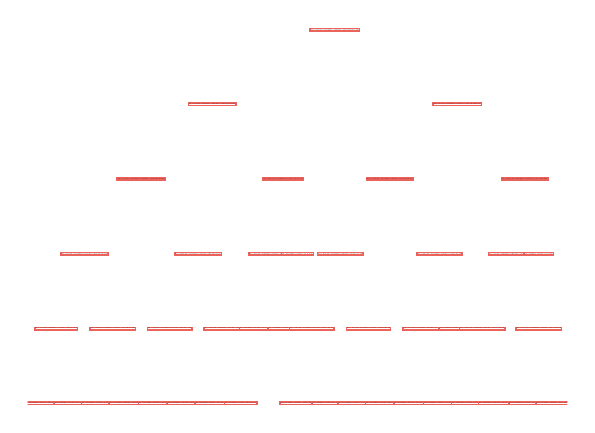
\begin{tikzpicture}

\definecolor{darkgray176}{RGB}{176,176,176}
\definecolor{tomato2369992}{RGB}{236,99,92}

\begin{axis}[
hide x axis,
hide y axis,
tick align=outside,
tick pos=left,
x grid style={darkgray176},
xmin=0, xmax=1,
xtick style={color=black},
y grid style={darkgray176},
ymin=0, ymax=1,
ytick style={color=black}
]
\draw (axis cs:0.0263157894736842,0.0833333333333333) node[
  scale=0.05,
  fill=white,
  draw=tomato2369992,
  line width=0.6pt,
  inner sep=3.6pt,
  text=black,
  rotate=0.0,
  align=center
]{gini = 0.059
samples = 5026
value = [4873, 15, 0, 138]};
\draw (axis cs:0.0789473684210526,0.0833333333333333) node[
  scale=0.05,
  fill=white,
  draw=tomato2369992,
  line width=0.6pt,
  inner sep=3.6pt,
  text=black,
  rotate=0.0,
  align=center
]{gini = 0.271
samples = 303
value = [256, 35, 0, 12]};
\draw (axis cs:0.131578947368421,0.0833333333333333) node[
  scale=0.05,
  fill=white,
  draw=tomato2369992,
  line width=0.6pt,
  inner sep=3.6pt,
  text=black,
  rotate=0.0,
  align=center
]{gini = 0.28
samples = 5586
value = [4653, 18, 10, 905]};
\draw (axis cs:0.184210526315789,0.0833333333333333) node[
  scale=0.05,
  fill=white,
  draw=tomato2369992,
  line width=0.6pt,
  inner sep=3.6pt,
  text=black,
  rotate=0.0,
  align=center
]{gini = 0.551
samples = 2404
value = [1505, 166, 232, 501]};
\draw (axis cs:0.236842105263158,0.0833333333333333) node[
  scale=0.05,
  fill=white,
  draw=tomato2369992,
  line width=0.6pt,
  inner sep=3.6pt,
  text=black,
  rotate=0.0,
  align=center
]{gini = 0.425
samples = 1254
value = [913, 256, 20, 65]};
\draw (axis cs:0.289473684210526,0.0833333333333333) node[
  scale=0.05,
  fill=white,
  draw=tomato2369992,
  line width=0.6pt,
  inner sep=3.6pt,
  text=black,
  rotate=0.0,
  align=center
]{gini = 0.581
samples = 1281
value = [614, 551, 36, 80]};
\draw (axis cs:0.342105263157895,0.0833333333333333) node[
  scale=0.05,
  fill=white,
  draw=tomato2369992,
  line width=0.6pt,
  inner sep=3.6pt,
  text=black,
  rotate=0.0,
  align=center
]{gini = 0.727
samples = 748
value = [157, 181, 130, 280]};
\draw (axis cs:0.394736842105263,0.0833333333333333) node[
  scale=0.05,
  fill=white,
  draw=tomato2369992,
  line width=0.6pt,
  inner sep=3.6pt,
  text=black,
  rotate=0.0,
  align=center
]{gini = 0.63
samples = 688
value = [343, 219, 35, 91]};
\draw (axis cs:0.5,0.0833333333333333) node[
  scale=0.05,
  fill=white,
  draw=tomato2369992,
  line width=0.6pt,
  inner sep=3.6pt,
  text=black,
  rotate=0.0,
  align=center
]{gini = 0.686
samples = 1928
value = [504, 826, 461, 137]};
\draw (axis cs:0.552631578947368,0.0833333333333333) node[
  scale=0.05,
  fill=white,
  draw=tomato2369992,
  line width=0.6pt,
  inner sep=3.6pt,
  text=black,
  rotate=0.0,
  align=center
]{gini = 0.0
samples = 24
value = [0, 0, 0, 24]};
\draw (axis cs:0.605263157894737,0.0833333333333333) node[
  scale=0.05,
  fill=white,
  draw=tomato2369992,
  line width=0.6pt,
  inner sep=3.6pt,
  text=black,
  rotate=0.0,
  align=center
]{gini = 0.676
samples = 334
value = [9, 85, 120, 120]};
\draw (axis cs:0.657894736842105,0.0833333333333333) node[
  scale=0.05,
  fill=white,
  draw=tomato2369992,
  line width=0.6pt,
  inner sep=3.6pt,
  text=black,
  rotate=0.0,
  align=center
]{gini = 0.718
samples = 414
value = [102, 158, 100, 54]};
\draw (axis cs:0.710526315789474,0.0833333333333333) node[
  scale=0.05,
  fill=white,
  draw=tomato2369992,
  line width=0.6pt,
  inner sep=3.6pt,
  text=black,
  rotate=0.0,
  align=center
]{gini = 0.29
samples = 3158
value = [52, 2637, 327, 142]};
\draw (axis cs:0.763157894736842,0.0833333333333333) node[
  scale=0.05,
  fill=white,
  draw=tomato2369992,
  line width=0.6pt,
  inner sep=3.6pt,
  text=black,
  rotate=0.0,
  align=center
]{gini = 0.61
samples = 301
value = [9, 152, 104, 36]};
\draw (axis cs:0.815789473684211,0.0833333333333333) node[
  scale=0.05,
  fill=white,
  draw=tomato2369992,
  line width=0.6pt,
  inner sep=3.6pt,
  text=black,
  rotate=0.0,
  align=center
]{gini = 0.404
samples = 416
value = [29, 36, 316, 35]};
\draw (axis cs:0.868421052631579,0.0833333333333333) node[
  scale=0.05,
  fill=white,
  draw=tomato2369992,
  line width=0.6pt,
  inner sep=3.6pt,
  text=black,
  rotate=0.0,
  align=center
]{gini = 0.202
samples = 7708
value = [349, 19, 6858, 482]};
\draw (axis cs:0.921052631578947,0.0833333333333333) node[
  scale=0.05,
  fill=white,
  draw=tomato2369992,
  line width=0.6pt,
  inner sep=3.6pt,
  text=black,
  rotate=0.0,
  align=center
]{gini = 0.544
samples = 193
value = [7, 23, 121, 42]};
\draw (axis cs:0.973684210526316,0.0833333333333333) node[
  scale=0.05,
  fill=white,
  draw=tomato2369992,
  line width=0.6pt,
  inner sep=3.6pt,
  text=black,
  rotate=0.0,
  align=center
]{gini = 0.332
samples = 2102
value = [121, 9, 1690, 282]};
\draw (axis cs:0.0526315789473684,0.25) node[
  scale=0.05,
  fill=white,
  draw=tomato2369992,
  line width=0.6pt,
  inner sep=3.6pt,
  text=black,
  rotate=0.0,
  align=center
]{X[1] <= 96.97
gini = 0.073
samples = 5329
value = [5129, 50, 0, 150]};
\draw (axis cs:0.157894736842105,0.25) node[
  scale=0.05,
  fill=white,
  draw=tomato2369992,
  line width=0.6pt,
  inner sep=3.6pt,
  text=black,
  rotate=0.0,
  align=center
]{X[1] <= 0.005
gini = 0.374
samples = 7990
value = [6158, 184, 242, 1406]};
\draw (axis cs:0.263157894736842,0.25) node[
  scale=0.05,
  fill=white,
  draw=tomato2369992,
  line width=0.6pt,
  inner sep=3.6pt,
  text=black,
  rotate=0.0,
  align=center
]{X[1] <= 253.08
gini = 0.532
samples = 2535
value = [1527, 807, 56, 145]};
\draw (axis cs:0.368421052631579,0.25) node[
  scale=0.05,
  fill=white,
  draw=tomato2369992,
  line width=0.6pt,
  inner sep=3.6pt,
  text=black,
  rotate=0.0,
  align=center
]{X[3] <= 213.58
gini = 0.721
samples = 1436
value = [500, 400, 165, 371]};
\draw (axis cs:0.421052631578947,0.25) node[
  scale=0.05,
  fill=white,
  draw=tomato2369992,
  line width=0.6pt,
  inner sep=3.6pt,
  text=black,
  rotate=0.0,
  align=center
]{gini = 0.457
samples = 147
value = [46, 0, 3, 98]};
\draw (axis cs:0.473684210526316,0.25) node[
  scale=0.05,
  fill=white,
  draw=tomato2369992,
  line width=0.6pt,
  inner sep=3.6pt,
  text=black,
  rotate=0.0,
  align=center
]{gini = 0.648
samples = 33
value = [15, 11, 1, 6]};
\draw (axis cs:0.526315789473684,0.25) node[
  scale=0.05,
  fill=white,
  draw=tomato2369992,
  line width=0.6pt,
  inner sep=3.6pt,
  text=black,
  rotate=0.0,
  align=center
]{X[5] <= 2502.5
gini = 0.692
samples = 1952
value = [504, 826, 461, 161]};
\draw (axis cs:0.631578947368421,0.25) node[
  scale=0.05,
  fill=white,
  draw=tomato2369992,
  line width=0.6pt,
  inner sep=3.6pt,
  text=black,
  rotate=0.0,
  align=center
]{X[3] <= 193.36
gini = 0.732
samples = 748
value = [111, 243, 220, 174]};
\draw (axis cs:0.736842105263158,0.25) node[
  scale=0.05,
  fill=white,
  draw=tomato2369992,
  line width=0.6pt,
  inner sep=3.6pt,
  text=black,
  rotate=0.0,
  align=center
]{X[1] <= 766.93
gini = 0.331
samples = 3459
value = [61, 2789, 431, 178]};
\draw (axis cs:0.789473684210526,0.25) node[
  scale=0.05,
  fill=white,
  draw=tomato2369992,
  line width=0.6pt,
  inner sep=3.6pt,
  text=black,
  rotate=0.0,
  align=center
]{gini = 0.0
samples = 113
value = [0, 0, 0, 113]};
\draw (axis cs:0.842105263157895,0.25) node[
  scale=0.05,
  fill=white,
  draw=tomato2369992,
  line width=0.6pt,
  inner sep=3.6pt,
  text=black,
  rotate=0.0,
  align=center
]{X[1] <= 811.925
gini = 0.214
samples = 8124
value = [378, 55, 7174, 517]};
\draw (axis cs:0.947368421052632,0.25) node[
  scale=0.05,
  fill=white,
  draw=tomato2369992,
  line width=0.6pt,
  inner sep=3.6pt,
  text=black,
  rotate=0.0,
  align=center
]{X[1] <= 815.565
gini = 0.354
samples = 2295
value = [128, 32, 1811, 324]};
\draw (axis cs:0.105263157894737,0.416666666666667) node[
  scale=0.05,
  fill=white,
  draw=tomato2369992,
  line width=0.6pt,
  inner sep=3.6pt,
  text=black,
  rotate=0.0,
  align=center
]{X[2] <= 47.88
gini = 0.268
samples = 13319
value = [11287, 234, 242, 1556]};
\draw (axis cs:0.315789473684211,0.416666666666667) node[
  scale=0.05,
  fill=white,
  draw=tomato2369992,
  line width=0.6pt,
  inner sep=3.6pt,
  text=black,
  rotate=0.0,
  align=center
]{X[2] <= 127.415
gini = 0.627
samples = 3971
value = [2027, 1207, 221, 516]};
\draw (axis cs:0.447368421052632,0.416666666666667) node[
  scale=0.05,
  fill=white,
  draw=tomato2369992,
  line width=0.6pt,
  inner sep=3.6pt,
  text=black,
  rotate=0.0,
  align=center
]{X[1] <= 202.7
gini = 0.547
samples = 180
value = [61, 11, 4, 104]};
\draw (axis cs:0.5,0.416666666666667) node[
  scale=0.05,
  fill=white,
  draw=tomato2369992,
  line width=0.6pt,
  inner sep=3.6pt,
  text=black,
  rotate=0.0,
  align=center
]{gini = 0.165
samples = 577
value = [36, 11, 4, 526]};
\draw (axis cs:0.578947368421053,0.416666666666667) node[
  scale=0.05,
  fill=white,
  draw=tomato2369992,
  line width=0.6pt,
  inner sep=3.6pt,
  text=black,
  rotate=0.0,
  align=center
]{X[2] <= 113.46
gini = 0.712
samples = 2700
value = [615, 1069, 681, 335]};
\draw (axis cs:0.763157894736842,0.416666666666667) node[
  scale=0.05,
  fill=white,
  draw=tomato2369992,
  line width=0.6pt,
  inner sep=3.6pt,
  text=black,
  rotate=0.0,
  align=center
]{X[5] <= 2502.5
gini = 0.369
samples = 3572
value = [61, 2789, 431, 291]};
\draw (axis cs:0.894736842105263,0.416666666666667) node[
  scale=0.05,
  fill=white,
  draw=tomato2369992,
  line width=0.6pt,
  inner sep=3.6pt,
  text=black,
  rotate=0.0,
  align=center
]{X[5] <= 52.5
gini = 0.247
samples = 10419
value = [506, 87, 8985, 841]};
\draw (axis cs:0.947368421052632,0.416666666666667) node[
  scale=0.05,
  fill=white,
  draw=tomato2369992,
  line width=0.6pt,
  inner sep=3.6pt,
  text=black,
  rotate=0.0,
  align=center
]{gini = 0.0
samples = 206
value = [0, 0, 0, 206]};
\draw (axis cs:0.210526315789474,0.583333333333333) node[
  scale=0.05,
  fill=white,
  draw=tomato2369992,
  line width=0.6pt,
  inner sep=3.6pt,
  text=black,
  rotate=0.0,
  align=center
]{X[1] <= 135.22
gini = 0.385
samples = 17290
value = [13314, 1441, 463, 2072]};
\draw (axis cs:0.473684210526316,0.583333333333333) node[
  scale=0.05,
  fill=white,
  draw=tomato2369992,
  line width=0.6pt,
  inner sep=3.6pt,
  text=black,
  rotate=0.0,
  align=center
]{X[5] <= 1067.5
gini = 0.29
samples = 757
value = [97, 22, 8, 630]};
\draw (axis cs:0.671052631578947,0.583333333333333) node[
  scale=0.05,
  fill=white,
  draw=tomato2369992,
  line width=0.6pt,
  inner sep=3.6pt,
  text=black,
  rotate=0.0,
  align=center
]{X[1] <= 563.315
gini = 0.569
samples = 6272
value = [676, 3858, 1112, 626]};
\draw (axis cs:0.921052631578947,0.583333333333333) node[
  scale=0.05,
  fill=white,
  draw=tomato2369992,
  line width=0.6pt,
  inner sep=3.6pt,
  text=black,
  rotate=0.0,
  align=center
]{X[5] <= 2502.5
gini = 0.273
samples = 10625
value = [506, 87, 8985, 1047]};
\draw (axis cs:0.342105263157895,0.75) node[
  scale=0.05,
  fill=white,
  draw=tomato2369992,
  line width=0.6pt,
  inner sep=3.6pt,
  text=black,
  rotate=0.0,
  align=center
]{X[5] <= 525.0
gini = 0.418
samples = 18047
value = [13411, 1463, 471, 2702]};
\draw (axis cs:0.796052631578947,0.75) node[
  scale=0.05,
  fill=white,
  draw=tomato2369992,
  line width=0.6pt,
  inner sep=3.6pt,
  text=black,
  rotate=0.0,
  align=center
]{X[1] <= 783.3
gini = 0.574
samples = 16897
value = [1182, 3945, 10097, 1673]};
\draw (axis cs:0.569078947368421,0.916666666666667) node[
  scale=0.05,
  fill=white,
  draw=tomato2369992,
  line width=0.6pt,
  inner sep=3.6pt,
  text=black,
  rotate=0.0,
  align=center
]{X[1] <= 385.71
gini = 0.695
samples = 34944
value = [14593, 5408, 10568, 4375]};
\end{axis}

\end{tikzpicture}
